\documentclass[aspectratio=169]{beamer}\usepackage[utf8]{inputenc}
\usepackage[english]{babel}
\usepackage{color}
\usepackage{amsmath,mathtools}
\usepackage{mathptmx}
\usepackage[11pt]{moresize}
\setbeamertemplate{navigation symbols}{}
\setbeamersize{text margin left=5mm,text margin right=5mm}
\usepackage{wrapfig}
\usepackage{bbm}
\usepackage{xcolor}
\usepackage{tabularx}
\usepackage{bm}
\usepackage{lmodern}


\newcommand{\R}{\mathbb{R}}
\newcommand{\E}{\mathbb{E}}
\newcommand{\N}{\mathbb{N}}
\newcommand{\Z}{\mathbb{Z}}
\newcommand{\V}{\mathbb{V}}
\newcommand{\Q}{\mathbb{Q}}
\newcommand{\K}{\mathbb{K}}
\newcommand{\C}{\mathbb{C}}
\newcommand{\T}{\mathbb{T}}
\newcommand{\I}{\mathbb{I}}

\setbeamertemplate{caption}[numbered]

\title{On the Uncertainty of Wind Power Generation\\ demo}
\subtitle{ Waleed Alhaddad}

\begin{document}
\setbeamercolor{background canvas}{bg=blue!1}


\begin{frame}{Uncertainty in Wind Power production}
Reliable wind power generation forecasting is crucial to:
\begin{itemize}
\item  Meet energy demand through renewable power sources.
\item  Energy trading of future excess power.
\item Design of Investment strategies.
\end{itemize}
We would like to:
\begin{itemize}
\item  Simulate forecast error and quantify its uncertainty.
\item  Calibrate a forecast model for  optimal dispatch of electric power.
\end{itemize}
Our model is based on:
\begin{itemize}
\item Parametric Stochastic Differential Equations.
\item Continuous optimization of approximate Maximum Likelihood.
\end{itemize}
\end{frame}



\begin{frame}{Uncertainty in Wind Power production}
\begin{minipage}{0.4\textwidth}
Prediction error of Wind Power production can be modeled by a parametric SDE,
		\begin{equation*}
		\begin{split}
		dV_t &=  - \theta_t V_t \  dt + \sqrt{2 \theta_t \alpha (V_t +p_t ) (1-V_t-p_t)} dW_t  \\ %\quad t > 0
		V_0 & = v_0
	\end{split}
	\end{equation*}
	where $V_t$ is an error stochastic process, $p_t$ is a given wind power forecast and $(\alpha, \theta)$ are parameters to the model
\end{minipage}%
\begin{minipage}{0.6\textwidth}
		\begin{figure}
			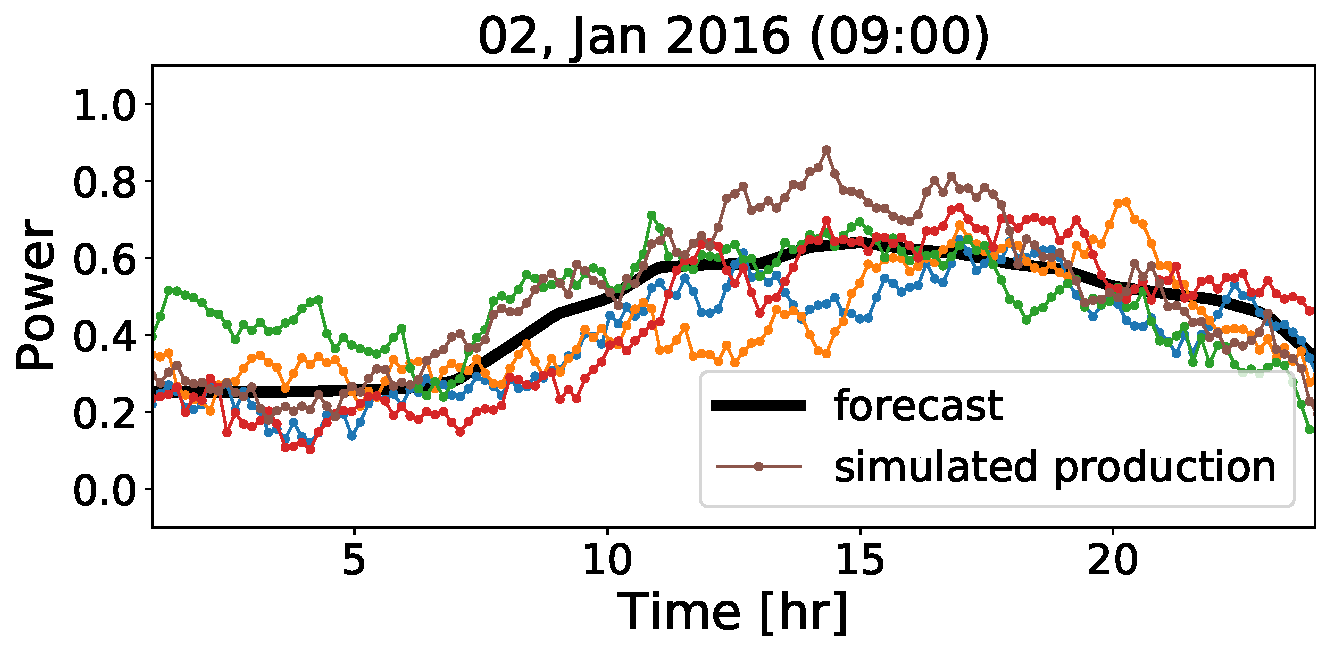
\includegraphics[width=0.7\linewidth]{plots_SGD/0.pdf}\\
			\hskip 125pt
			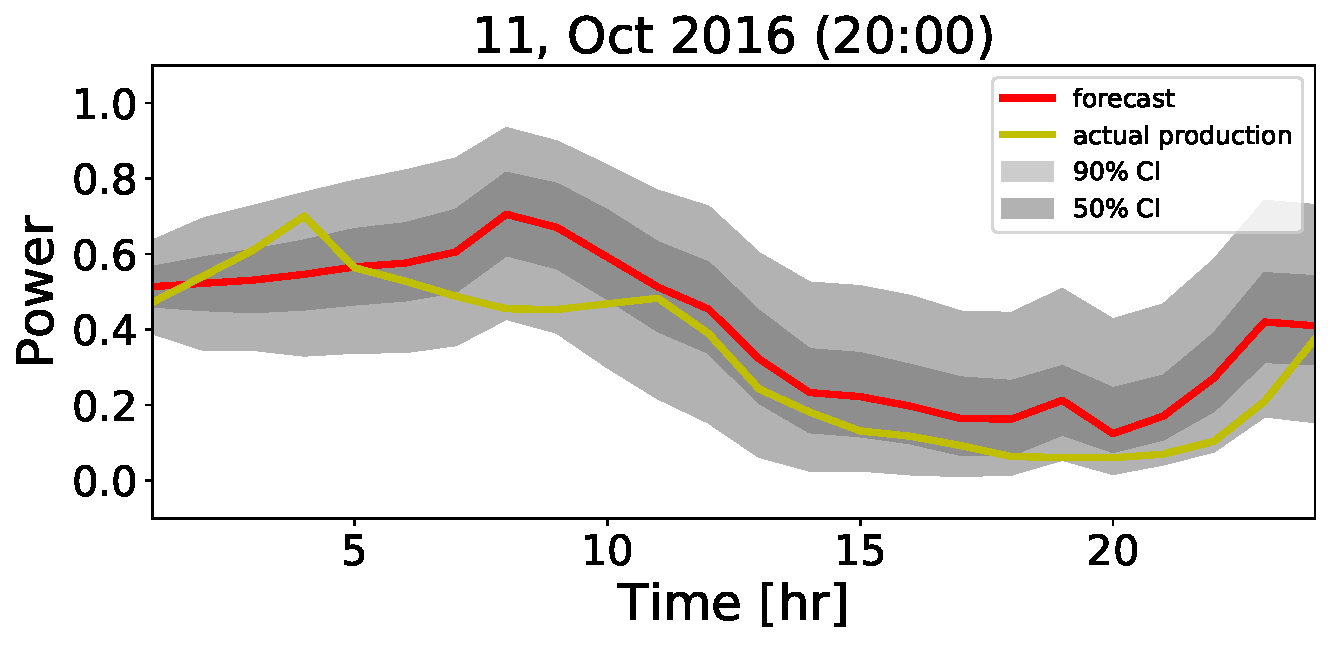
\includegraphics[width=0.7\linewidth]{plots_SGD/820.pdf}
			\caption{Example of Wind power production simulation and confidence intervals.}
			\end{figure}
\end{minipage}
\end{frame}


\begin{frame}\frametitle{Uncertainty in Wind Power production}
\noindent
\begin{minipage}[t]{0.5\textwidth}
\hskip 10pt
Parameters of the model are inferred using optimization techniques of approximate transition likelihood functions.
\begin{equation*}
\mathcal{L}(\bm{\theta};V) =\prod\limits_{j=1}^M \prod\limits_{i=1}^N \rho ( {V_{j,i+1}|V_{j,i}}, \bm{\theta})  \rho (V_{j,0})
\end{equation*}
Where  $ V^{M,N}=\{ V_{t_1^{M,N}} , V_{t_2^{M,N}} ,\ldots , V_{t_N^{M,N}} \}$ is a set of M paths with N observations observed in intervals of time $\Delta_N$.
\end{minipage}%
\begin{minipage}[t]{0.5\textwidth}
\begin{figure}
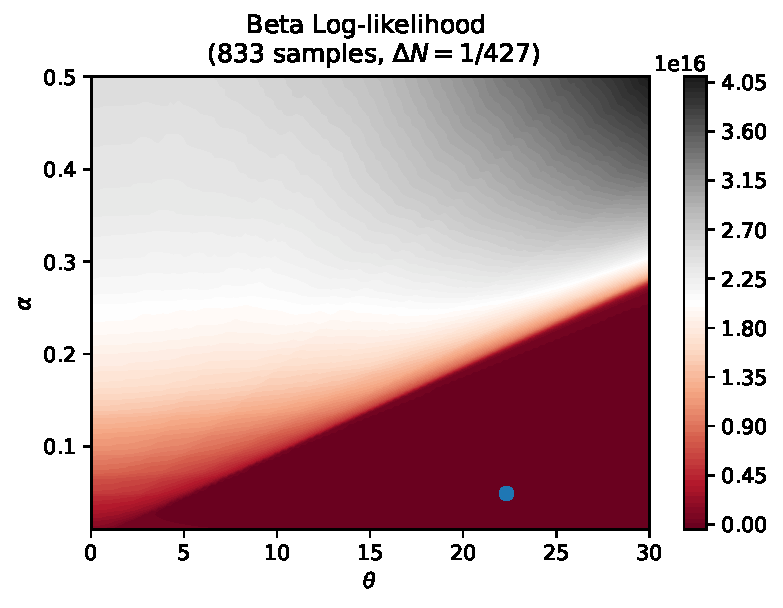
\includegraphics[width=0.8\linewidth]{plots_SGD/ISO_833_inter=427.pdf}
   \caption{Likelihood of sample paths. Point of optimality shown in blue.}
\label{samples}
\end{figure}
\end{minipage}
\end{frame}

\end{document}
